\item[6] Consider a triangle $ABC$. Each angle is split a line segment, that all intersect at a common point $O$ somewhere within the circle, but not exactly on any of the sides $AB$, $BC$, or $AC$. An example is shown in the figure below.

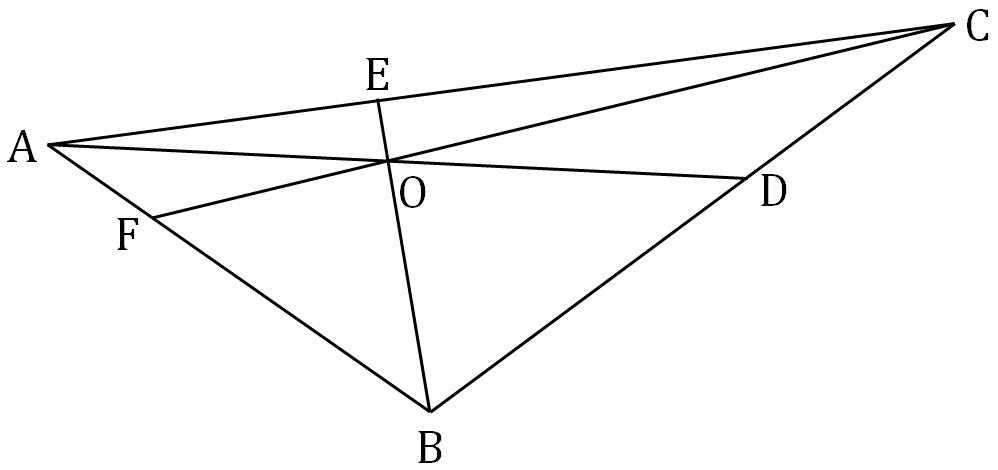
\includegraphics[height=3.5cm]{images/triangle.png}

Is it possible to draw a triangle, with a common point $O$ somewhere inside the triangle (but not exactly on the sides) such that $\frac{AF}{FB}\cdot \frac{BD}{DC} \cdot \frac{CE}{EA} \neq 1$? In this equation above, $XY$ means the length of the line segment created by the points $X$ and $Y$. Explain how to draw such a triangle and the common point $O$, or prove that the product of the specified ratios is always equal to 1. Hint: try to relate side lengths to area, and try to find relations between ratios/sums/differences of side lengths and areas of different triangles.
  \begin{Questions}
  \\
  \\
  {\color{NavyBlue}
  \\ We can define x, y as any x and y coordinate of O, and WithinABC(x, y) as a function that produces true if the coordinates land inside triangle ABC defined in the illustration above, and false otherwise.
  \\ $\forall x, y \in \R, WithinABC(x, y) \rightarrow \frac{\overline{AF}}{\overline{FB}}\cdot \frac{\overline{BD}}{\overline{  DC}} \cdot \frac{\overline{  CE}}{\overline{  EA}} = 1$
  \\
  \\Proof:
  \\It is not possible since all positions of O will yield make $\frac{\overline{AF}}{\overline{FB}}\cdot \frac{\overline{BD}}{\overline{  DC}} \cdot \frac{\overline{  CE}}{\overline{  EA}} = 1$ true. 
  \\
  \\There are two equations for an area of a triangle, where a, b, c are the sides of the triangle, and A, B, C are the angles of the triangle, corresponding respectively:
  \\
  \\Area = (1/2)ab(sinC) = (1/2)ch
  \\Where h is a line that is perpendicular to c and intersects the intersection between a and b.
  \\
  \\To apply these formulas to this question, we have to label the triangle with more points, so we can draw "h" to satisfy "Area = (1/2)ch" for all triangles:
  \\
  \\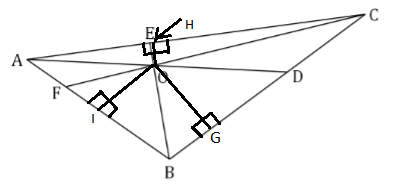
\includegraphics[height=4.0cm]{q4.PNG}
  \\
  \\We can use these new points to write out the area formulas for the given triangles. I will be using $\triangle$ as shorthand for "Area of", $\angle$ for "Angle of", a line above characters for "Segment of", and [n] besides the question to number the corresponding equation. Note that the ordering of the letters does not matter (for example, $\overline{AO} = \overline{OA}$):
  \\
  \\$[1]\triangle AOF = (1/2)*\overline{AO}*\overline{FO}*sin(\angle AOF)$
  \\$[2]\triangle AOF = (1/2)*\overline{AF}*\overline{IO}$
  \\$[3]\triangle FOB = (1/2)*\overline{FO}*\overline{BO}*sin(\angle FOB)$
  \\$[4]\triangle FOB = (1/2)*\overline{FB}*\overline{IO}$
  \\$[5]\triangle BOD = (1/2)*\overline{BO}*\overline{DO}*sin(\angle BOD)$
  \\$[6]\triangle BOD = (1/2)*\overline{BD}*\overline{GO}$  \\$[7]\triangle DOC = (1/2)*\overline{DO}*\overline{CO}*sin(\angle DOC)$
  \\$[8]\triangle DOC = (1/2)*\overline{DC}*\overline{GO}$  \\$[9]\triangle COE = (1/2)*\overline{CO}*\overline{EO}*sin(\angle COE)$
  \\$[10]\triangle COE = (1/2)*\overline{CE}*\overline{HO}$
  \\$[11]\triangle AOE = (1/2)*\overline{AO}*\overline{EO}*sin(\angle AOE)$
  \\$[12]\triangle AOE = (1/2)*\overline{AE}*\overline{HO}$
  \\
  \\Note that because $\overline{AD}$ and $\overline{FC}$ are straight and intersect to create $\triangle AOF$ and $\triangle COD$, $\triangle AOF$ and $\triangle COD$ are equal due to properties of vertically opposite angles. This also applies to $\triangle FOB$ and $\triangle EOC$, as well as $\triangle BOD$ and $\triangle AOE$. This gives use three more equations:
  \\
  \\$[13]\triangle AOF = \triangle COD$
  \\$[14]\triangle FOB = \triangle COE$
  \\$[15]\triangle BOD = \triangle AOE$
  \\
  \\To prove that $\frac{\overline{AF}}{\overline{FB}}\cdot \frac{\overline{BD}}{\overline{  DC}} \cdot \frac{\overline{  CE}}{\overline{  EA}} = 1$ is true, it is useful to prove that $\frac{\triangle AOF}{\triangle FOB}\cdot \frac{\triangle BOD}{\triangle DOC} \cdot \frac{\triangle COE}{\triangle EOA} = 1$, or in other words $\triangle AOF *\triangle BOD * \triangle COE=\triangle FOB*\triangle DOC*\triangle EOA$ is true. We get this as a result:
  \\ 
  \\$\triangle AOF *\triangle BOD * \triangle COE=\triangle FOB*\triangle DOC*\triangle EOA$ [Start]
  \\$(1/2)*\overline{AO}*\overline{FO}*sin(\angle AOF) * (1/2)*\overline{BO}*\overline{DO}*sin(\angle BOD)* (1/2)*\overline{CO}*\overline{EO}*sin(\angle COE) = (1/2)*\overline{FO}*\overline{BO}*sin(\angle FOB)* (1/2)*\overline{DO}*\overline{CO}*sin(\angle DOC) (1/2)*\overline{AO}*\overline{EO}*sin(\angle AOE)$ [Substitution from equations 1,3,5,7,9,11]
  \\$(1/2)*\overline{AO}*\overline{FO}*sin(\angle DOC) * (1/2)*\overline{BO}*\overline{DO}*sin(\angle AOE)* (1/2)*\overline{CO}*\overline{EO}*sin(\angle FOB) = (1/2)*\overline{FO}*\overline{BO}*sin(\angle FOB)* (1/2)*\overline{DO}*\overline{CO}*sin(\angle DOC) (1/2)*\overline{AO}*\overline{EO}*sin(\angle AOE)$ [Substitution from equations 13,14,15]
  \\$(1/2)*(1/2)*(1/2)\overline{AO}*\overline{BO}*\overline{CO}*\overline{DO}*\overline{EO}*\overline{FO}*sin(\angle FOB)*sin(\angle DOC)*sin(\angle AOE) = (1/2)*(1/2)*(1/2)\overline{AO}*\overline{BO}*\overline{CO}*\overline{DO}*\overline{EO}*\overline{FO}*sin(\angle FOB)*sin(\angle DOC)*sin(\angle AOE)$ [Reordering of terms to make equating more obvious]
  \\
  \\Thus, we have proved that $\frac{\triangle AOF}{\triangle FOB}\cdot \frac{\triangle BOD}{\triangle DOC} \cdot \frac{\triangle COE}{\triangle EOA} = 1$ is true. To prove that $\frac{\overline{AF}}{\overline{FB}}\cdot \frac{\overline{BD}}{\overline{  DC}} \cdot \frac{\overline{  CE}}{\overline{  EA}} = 1$ is true, we have to substitute equations 2,4,6,8,10,12 into the proven area equating equation:
  \\
  \\$\frac{\triangle AOF}{\triangle FOB}\cdot \frac{\triangle BOD}{\triangle DOC} \cdot \frac{\triangle COE}{\triangle EOA} = 1$ [Start]
  \\$\frac{(1/2)*\overline{AF}*\overline{IO}}{(1/2)*\overline{FB}*\overline{IO}}\cdot \frac{(1/2)*\overline{BD}*\overline{GO}}{(1/2)*\overline{DC}*\overline{GO}} \cdot \frac{(1/2)*\overline{CE}*\overline{HO}}{(1/2)*\overline{AE}*\overline{HO}} = 1$ [Substitution from equations 2,4,6,8,10,12]
  \\$\frac{\overline{AF}}{\overline{FB}}\cdot \frac{\overline{BD}}{\overline{  DC}} \cdot \frac{\overline{  CE}}{\overline{  EA}} = 1$ [Cancellation of all $(1/2),\overline{IO},\overline{GO},\overline{HO}$ terms]
  \\
  \\Therefore, we prove that it is not possible to draw a triangle, with a common point $O$ somewhere inside the triangle (but not exactly on the sides), such that $\frac{AF}{FB}\cdot \frac{BD}{DC} \cdot \frac{CE}{EA} \neq 1$, since $\frac{\overline{AF}}{\overline{FB}}\cdot \frac{\overline{BD}}{\overline{  DC}} \cdot \frac{\overline{  CE}}{\overline{  EA}} = 1$ is true for any arbitrary point.
  \\
  \\\boxed{}
  }
  \vfill\eject
  \end{Questions}